\documentclass[a4paper, 12pt]{article}%тип документа

%отступы
\usepackage[left=1.5cm,right=1cm,top=2cm,bottom=3cm,bindingoffset=0cm]{geometry}
\setlength{\parindent}{5ex}

%Русский язык
\usepackage[T2A]{fontenc} %кодировка
\usepackage[utf8]{inputenc} %кодировка исходного кода
\usepackage[english,russian]{babel} %локализация и переносы

%Вставка картинок
\usepackage{graphicx}
\graphicspath{{pictures/}}
\DeclareGraphicsExtensions{.pdf,.png,.jpg,}
\usepackage{wrapfig}

%Графики
\usepackage{pgfplots}
\pgfplotsset{compat=1.9}

%Математика
\usepackage{amsmath, amsfonts, amssymb, amsthm, mathtools}

%Таблицы
\usepackage{longtable} 
\usepackage{float}

%Римские цифры
\newcommand{\RomanNumeralCaps}[1]{\uppercase\expandafter{\romannumeral#1}}

\usepackage{multirow}


\begin{document}
	\begin{titlepage}
		\begin{center}
			\textsc{Федеральное государственное автономное образовательное учреждение высшего образования«Московский физико-технический институт (национальный исследовательский университет)»\\[5mm]
			}
			
			\vfill
			
			\textbf{Лабораторная работа: \\[3mm]
				Генерация второй гармоники
				\\[50mm]
			}
			
		\end{center}
		
		\hfill
		\begin{minipage}{.5\textwidth}
			Выполнили студенты:\\[2mm]
			Сериков Василий Романович\\[2mm]
			Группа: Б03-102\\[5mm]
			Сериков Алексей Романович\\[2mm]
			Группа: Б03-102\\[5mm]
			
		\end{minipage}
		\vfill
		\begin{center}
			Москва, 2024 г.
		\end{center}
		
	\end{titlepage}
	
	\newpage
	\textbf{Аннотация}\\
	
	В работе предлагается изучить нелинейно-оптическое явление - генерация второй гармоники.\\
	
	\textbf{Теоретические сведения: }\\
	
	При прохождении света через объем диэлектрика возникает ненулевая поляризуемость вещества. В классическом представлении колебание электронного облака атома приводит к переизлучению света на той же частоте что и у падающего излучения, что объясняется моделью осциллятора Лорентца для вещества. В общем случае поляризуемость вещества линейно зависит от прилагаемого поля и выражается следующим образом:
	\begin{equation}
		\vec{P} = \hat{\alpha}\vec{E},
	\end{equation}
	где $\hat{\alpha}$ - тензор восприимчивости. Видно, что в общем случае в линейном приближении вектор поляризации неколлинеарен напряженности поля.
	\par Однако при больших полях порядка $10^{5} - 10^{8}$ B/см проявляются нелинейные эффекты, приводящие к квадратичным и кубическим зависимостям поляризуемости от напряженности поля.
	\begin{equation}
		P_i = \alpha_{ik}E^k + A_{ijk}E^jE^k,
	\end{equation}
	где $A_{ijk}$ - тензор нелинейной восприимчивости 
	Подставим выражение для поля, меняющегося по гармоническому закону, $\vec{E} = E\cos(\omega t - kz)$, получим:
	\begin{equation}
		P_i = \alpha_{ik}E^k\cos(\omega t - kz) + \frac{1}{2}A_{ijk}E^jE^k + A_{ijk}E^jE^k\cos(2(\omega t - kz))
	\end{equation}
	Видим, что появляется слагаемое, меняющееся по гармоническому закону с удвоенной частотой, следовательно, будет происходить переизлучение света с удвоенной частотой.
	\par В нашей работе рассматриваем явление генерации второй гармоники в одноосном кристалле ниобата лития. Если падающая волна - обыкновенная, переизлученная - необыкновенная, то в случае отсутствия пространственного разделения волн набегает разность фаз $\Delta\phi = l(k_2 - 2k_1)$. Условие фазового синхронизма $\Delta\phi =0$
	\begin{equation}
		\vec{k_2} = 2\vec{k_1}, \quad n(\omega) = n(2\omega)
	\end{equation}
	
	\newpage
	
	\textbf{Ход работы: }\\
	
	Для кристалла ниобата лития приведем значения показателей преломления для обыкновенной и необыкновенной волн при частотах лазерного излучения, используемого в работе.

	
	\begin{longtable}{|c|c|c|}
		\hline
		$\lambda$, $\mu m$ & $n_0$ & $n_e$ \\
		\hline
		1.06 & 2.2336 & 2.1540 \\
		\hline
		0.53 & 2.3225 & 2.2289 \\
		\hline
		\caption{Показатели преломления для необыкновенной и обыкновенной волн в кристалле $LiNbO_3$}
	\end{longtable}

	\par При определенном падении волны, показатель преломления необыкновенной будет равен показателю для обыкновенной, что иллюстрирует рисунок 1 
	\begin{figure}[h!]
		\centering
		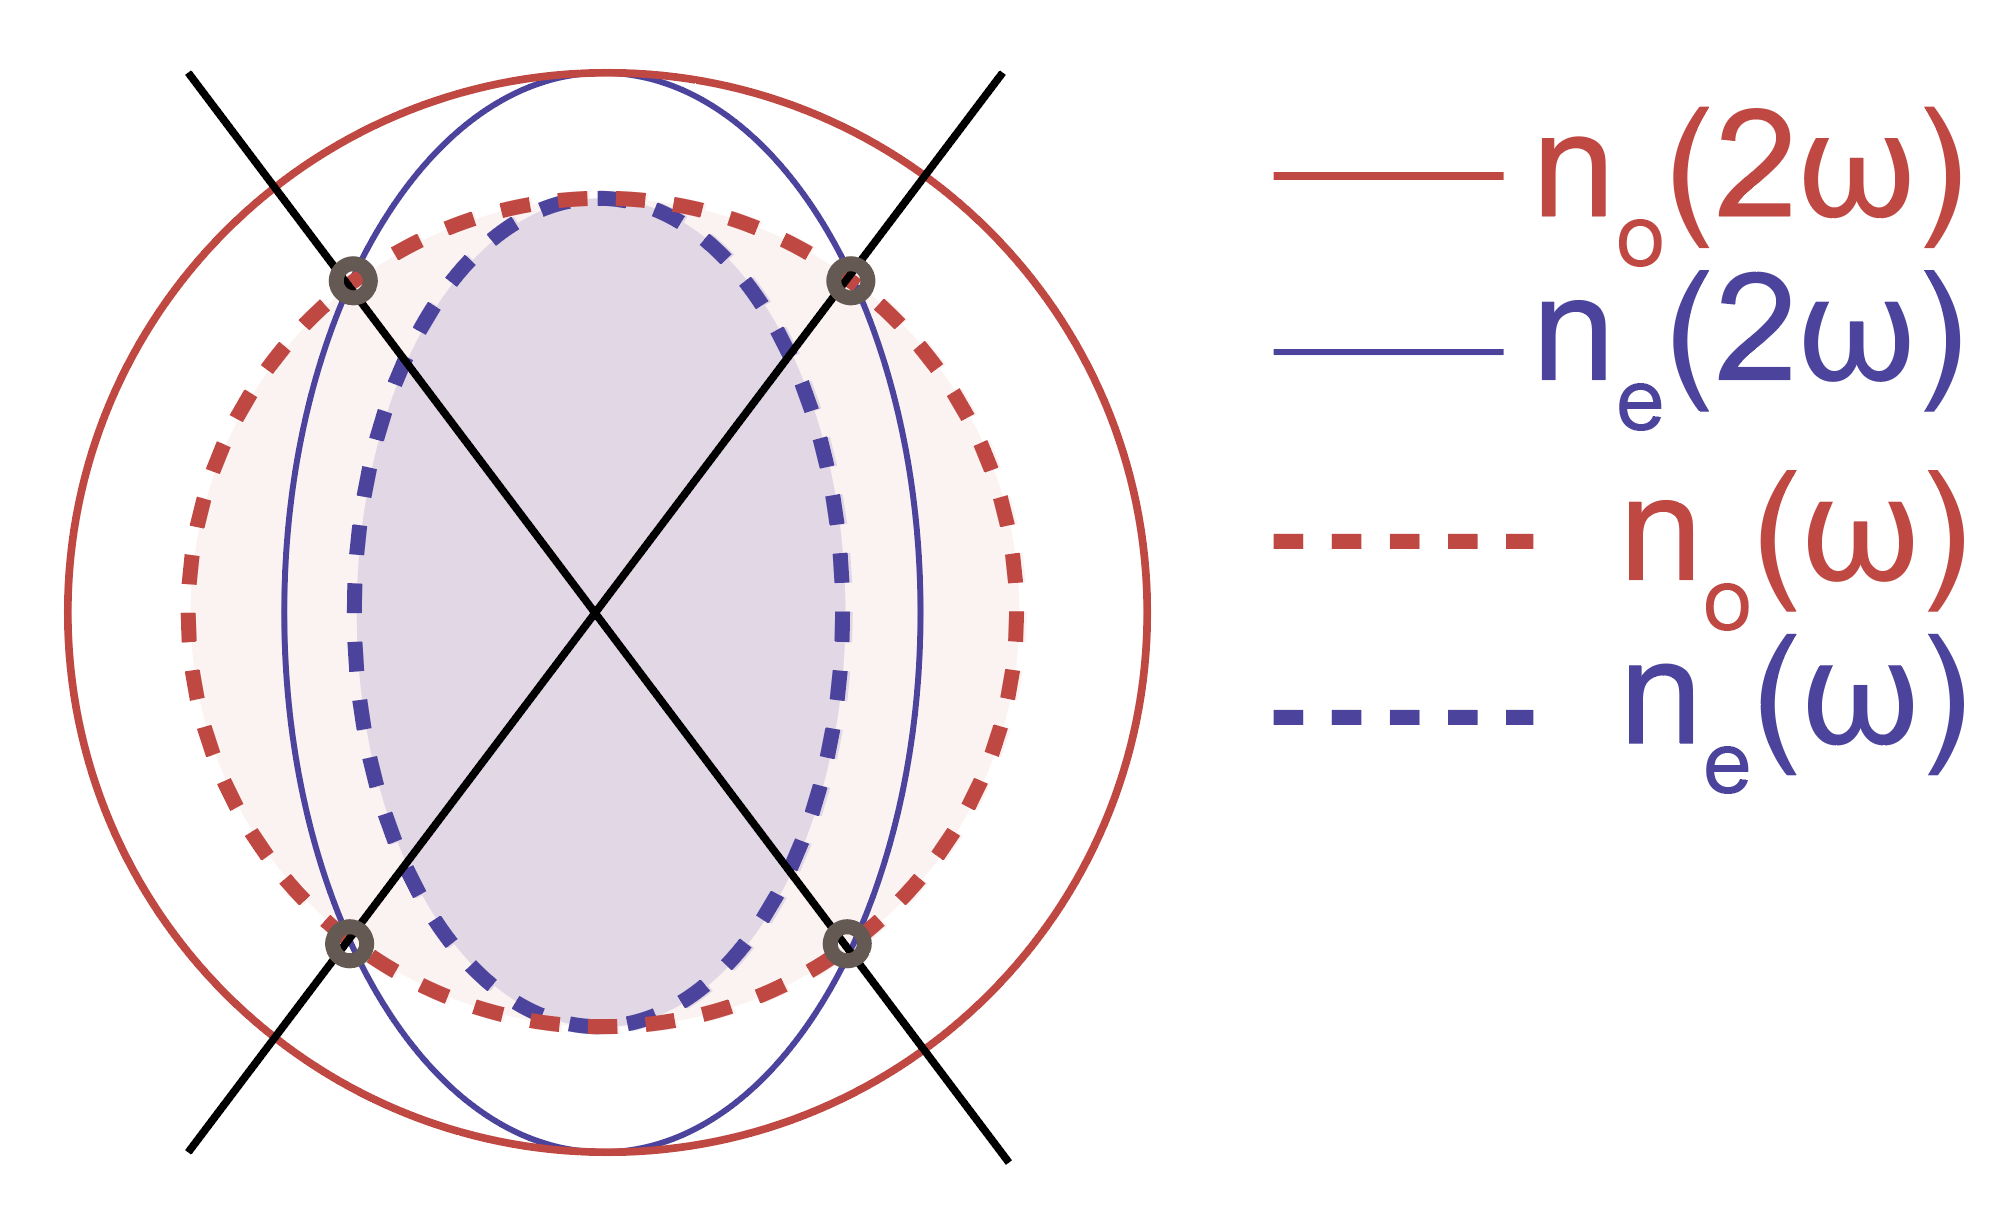
\includegraphics[width=0.7\linewidth]{Sinhronismwiki.png}
		\caption{Условие возникновения фазового синхронизма}
	\end{figure}
	Зависимость показателя преломления для необыкновенной волны от угла между вектором напряженности и оптической оси кристалла имеет вид:
	\begin{equation}
		n_e(\theta)  = \frac{n_o(2\omega)}{\sqrt{1 + ((\frac{n_o(2\omega)}{n_e(2\omega)})^2 - 1)\sin^2{\theta}}}, \quad n_o = const
	\end{equation}
	Выразив из последнего выражения $\theta$, мы получим угол между вектором напряженность и оптической осью кристалла, при котором наблюдается фазовый синхронизм
	\begin{equation}
		\theta_{0} = 90^{o}
	\end{equation}
	
	
	Определим ноль отсчета гониометра, для этого ориентируем кристалл так, чтобы луч, прошедший диафрагму, отразился от боковой поверхности кристалла и вновь попал на диафрагму. Таким образом мы сориентируем кристалл оптической осью вдоль распространения лазерного пучка. От этого положения будем отсчитывать все последующие углы.\\
	
	\begin{longtable}{|c|c|c|c|}
		\hline
		\multicolumn{4}{|c|}{Значение с гониометра, $^{o}$}\\
		\hline
		$351^{o}10'$&$351^{o}22'$&$351^{o}31'$&$351^{o}29'$ \\
		\hline
		\multicolumn{4}{|c|}{Среднее значение, $^{o}$}\\
		\hline
		\multicolumn{4}{c}{$351^{o}23'$}\\
		\hline
		\caption{Результаты калибровки}
	\end{longtable}

	\par Установим поляризатор на входе в двух положениях, когда пропускается только горизонтальная или вертикальная поляризация, снимем показания гониометра.
	
	\begin{longtable}{|c|c|c|c|}
			\hline
			$46^o03'$& $137^o01'$&$225^o49'$ &$320^o55'$\\
			\hline
		\caption{Полученные результаты углов синхронизма для горизонтальной поляризации}
	\end{longtable}
	
	\begin{longtable}{|c|c|c|c|}
		\hline
		$46^o0'$&$137^o07' $&$226^o01' $&$321^o20'$\\
		\hline
		\caption{Полученные результаты углов синхронизма для вертикальной поляризации}
	\end{longtable}
	
	
	\newpage
	\par Снимем распределение интенсивности в зависимости от угла вблизи максимума интенсивности рисунок 2
	
	\begin{figure}[H]
		\centering
		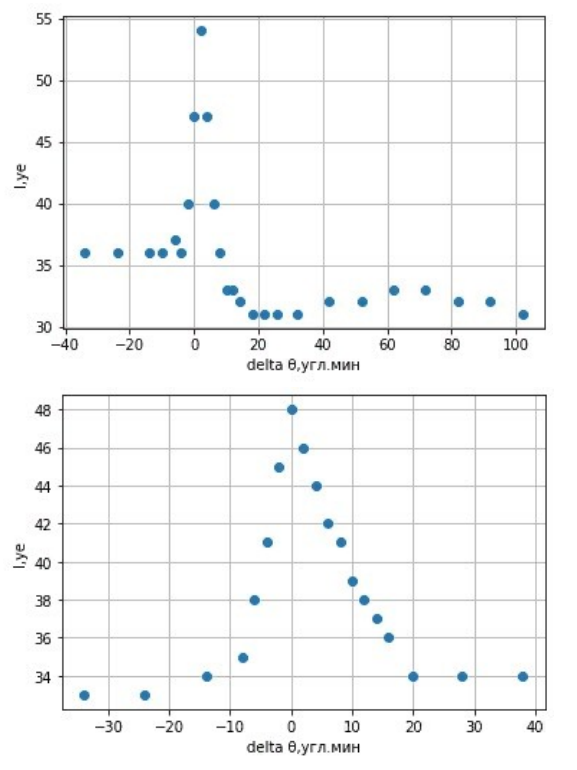
\includegraphics[width=0.6\linewidth]{graph.png}
		\caption{Зависимость интенсивности от углового смещения вблизи максимума}
		\label{fig:enter-label}
	\end{figure}
	
	\textbf{Результаты: }\\
	
	В ходе работы познакомились с явлением генерации второй гармоники в кристалле ниобата лития и сняли зависимость интенсивности от углового смещения.
	
	
	
	
	
	
	
	
	
	
	\end{document}